\chapter{Background}\label{background}
Fluid-structure interaction (FSI) problems in general are often too complex to solve analytically and so they have to be analyzed by means of experiments or numerical simulation. Although the maturity of the computational fluid dynamics enables numerical simulation of fluid structure interaction, considering turbulence flow in these problems adds more difficulties and challenges. The numerical models for solving FSI problems usually involve solving several equations describing the behaviors of fluid and structures. Sometimes the equations of the scalar field, such as temperature or the concentration of chemical species, also need to be considered as a significant component of the system. In this chapter, three different categories of equations for incompressible fluid, scalar field and particle dynamics are introduced in the mathematics point of view.

\section{Navier-Stokes equation and turbulent flow}
It is common to view turbulent flows in both our daily life, such as smoke from a chimney, water in a river, and engineering fields, such as flows around airplanes, or mixing of fuel and air in engines. In these observations, the flow is unsteady, irregular and chaotic. The motion of every eddy or droplet is unpredictable \cite{PopeTurbulent2000}. In another word, the velocity of turbulent flows varies irregularly in both position and time. The velocity field is denoted in mathematics by $\vect{U}(\vect{x},t)$, where $\vect{x}$ is the position and $t$ is time. Another important feature of turbulence is its ability to transport and mix fluid much more effectively than a comparable laminar flow. The intensity of turbulent flow is often characterized by a single non-dimensional parameter, Reynolds number\cite{Reynolds1894}: 
\begin{equation}
Re = U L / \nu
\label{ReynoldsNumber}
\end{equation}
where $U$ and $L$ are characteristic velocity and length scale of the flow, and $\nu$ is the kinematic viscosity of the fluid. According to Reynolds's experiment, the flow is laminar if $Re$ is less than about $2300$, and becomes turbulent if $Re$ exceeds $4000$.

A classic way to study fluid dynamics is to treat 
the fluids as continuous media, based on the continuum hypothesis, 
which reconciles the discrete molecular nature of fluids with the 
continuum view. Since the length and time scales of the molecular 
motion are extremely small compared with human scales, the fluid's velocity $\mathbf{U}(\mathbf{x}, t)$ is defined as the average velocity of the molecules within a spherical region of 
volume $V$ centered on the point $\mathbf{x}$. According to the conservation law of mass and momentum, the flow of constant property Newtonian fluids is determined by the 
following partial differential equations (PDE):
\begin{equation}
\frac{\partial\rho}{\partial t} + \nabla\cdot(\rho\mathbf{U}) = 0
\label{mass_eqn}
\end{equation} 

\begin{equation}
\frac{\partial\mathbf{U}}{\partial t} 
+ \mathbf{U}\cdot\nabla\mathbf{U} 
= -\frac{1}{\rho}\nabla p + \nu\nabla^2\mathbf{U}
\label{mom_eqn}
\end{equation}
where $\nu$ is the kinematic viscosity and $p$ is the pressure field. The above equations are usually called the Navier-Stokes equation. In this paper, we only consider constant density flows, and therefore \Eq{mass_eqn} degenerates to the divergence-free condition \cite{blazek2015computational}:
\begin{equation}
\nabla\cdot\mathbf{U} = 0
\label{div_free}
\end{equation}

The boundary conditions are essential for solving the above equations. At a stationary solid wall with unit normal $\mathbf{n}$, 
the boundary conditions are the impermeability condition \cite{blazek2015computational}
\begin{equation}
\mathbf{n}\cdot\mathbf{U} = 0
\label{imperm_cond}
\end{equation}
and the no-slip condition \cite{blazek2015computational}
\begin{equation}
\mathbf{U}-\mathbf{n}(\mathbf{n}\cdot\mathbf{U}) = 0
\label{noslip_cond}
\end{equation}
which together yield
\begin{equation}
\mathbf{U} = 0
\label{stat_cond}
\end{equation}

It is sometimes reasonable to assume the hypothetical case of an infinite domain, which is defined to have the periodic boundary condition. This condition is useful for approximating a large system by using a small unit cell \cite{blazek2015computational}. 

It is true that the fluid motion of laminar and turbulent flows can be determined by the Navier-Stokes equation. It appears that if one can solve the \Eq{mom_eqn} and \Eq{div_free}, either analytically or numerically, then the behavior of the fluid flow can be predicted. However, solving the Navier-Stokes equations remains an immensely challenging problem. Firstly, until now no one has ever been able to prove that smooth solution always exist, or that if they do exist, they have bounded energy per unit mass. This in called the Navier-Stokes existence and smoothness problem \cite{ladyzhenskaya1969mathematical} and has not been solved yet. On the other hand, although many well-understood numerical methods have existed for a long time and can be used to solve the PDEs like \Eq{mom_eqn} and \Eq{div_free}, massive computing resources are always needed to resolve all scales in a turbulent fluid: from energy containing scale to inertial sub-range, and down to the scale of viscous dissipation \cite{PopeTurbulent2000}. Failing to resolve the complete range of the length scales may result in unphysical numerical results. To obtain solutions for moderately high Reynolds numbers using the brutal-force approach, Directed Numerical Simulation (DNS) \cite{PopeTurbulent2000}, requires weeks of computing time on today's largest supercomputers. 

An alternative approach introduced by Osborne Reynolds in the late 19th century is to ignore the details of the turbulent flow at each instant and, instead, to regard the flow as a superposition of mean and fluctuating parts. According to the Reynolds decomposition \cite{PopeTurbulent2000}, the velocity $\mathbf{U}(\mathbf{x}, t)$ is decomposed into its mean $\langle\mathbf{U}(\mathbf{x},t)\rangle$ and the fluctuation $\mathbf{u}(\mathbf{x},t)$:
\begin{equation}
\mathbf{U}(\mathbf{x},t) = \langle\mathbf{U}(\mathbf{x},t)\rangle + \mathbf{u}(\mathbf{x},t)
\label{reynolds_decomp}
\end{equation}
Taking the mean of the divergence-free condition \Eq{div_free} and momentum equation \Eq{mom_eqn} yields the Reynolds Averaged Navier-Stokes(RANS) equations \cite{reynolds1894dynamical}:
\begin{equation}
\nabla\cdot\langle\mathbf{U}\rangle = 0
\label{div_free_U}
\end{equation}
\begin{equation}
\frac{\partial \langle U_j\rangle}{\partial t} + \langle \mathbf{U}\rangle
\cdot \nabla\langle U_j\rangle = 
- \frac{1}{\rho}\frac{\partial \langle p\rangle}{\partial x_j} + \nu\nabla^2\langle U_j\rangle - \frac{\partial\langle u_iu_j\rangle}{\partial x_i}
\label{reynolds_eqn}
\end{equation}
It is obvious that the Reynolds equations \Eq{reynolds_eqn} resembles the Navier-Stokes equation \Eq{mom_eqn} except the term of Reynolds stresses $\frac{\partial\langle u_iu_j\rangle}{\partial x_i}$ \cite{PopeTurbulent2000}, which plays a crucial role to distinguish the behaviors of $\mathbf{U}(\mathbf{x},t)$ and $\langle\mathbf{U}(\mathbf{x},t)\rangle$. The equation \Eq{reynolds_eqn} is incomplete since the Reynolds stresses appear as unknowns and are need to be determined by a turbulence model. The turbulent-viscosity models are based on the turbulent-viscosity hypothesis \cite{schmitt2007boussinesq}: 
\begin{equation}
\langle u_iu_j\rangle = \frac{2}{3}k\delta_{ij} 
- \nu_T(\frac{\partial\langle U_i\rangle}{\partial x_j} + 
\frac{\partial\langle U_j\rangle}{\partial x_i})
\label{visc_hypo}
\end{equation}   
where $k = 1/2\langle u_iu_i\rangle$ is the turbulent kinetic energy, $\delta_{ij}$ equals one when $i = j$ and zero otherwise. Given the turbulent eddy viscosity $\nu_T$ \cite{PopeTurbulent2000}, \Eq{visc_hypo} provides a convenient closure to the Reynolds equations. Although the accuracy of this hypothesis is poor for many flows \cite{PopeTurbulent2000}, this approach is widely accepted as an adequate approximation and has been applied to many studies involving turbulent flows. The turbulent viscosity $\nu_T(\mathbf{x},t)$ can be determined in many ways through defining different turbulence models, such as algebraic models \cite{baldwin1978thin}, one-equation models \cite{spalart1992one} and two-equation models \cite{WilcoxTurbulence2006}. In consideration of accuracy and efficiency, the RANS model is used only if the Reynolds number is extremely large and hence the computational cost can not be handled by the current computational resources. In this paper, DNS is used to study the homogeneous turbulence flow in a very small domain while RANS is adopted to study the problem with a much larger scale.   

\section{Convection-diffusion-reaction equation}
A scalar field, such as temperature, water vapor or the concentration of a chemical species, is often accompanied with the turbulent velocity $\mathbf{U}(\mathbf{x},t)$ in a real physics problem. In addition, the turbulence kinetic energy $k$ \cite{PopeTurbulent2000} and energy dissipation rate $\varepsilon$ \cite{PopeTurbulent2000}, which are related to the turbulent viscosity, can also be regarded as scalar fields. In a constant-property flow, the transport equation for a scalar field $\Phi$ is:
\begin{equation}
\frac{\partial\Phi}{\partial t} + \mathbf{U}\cdot\nabla\Phi = D\nabla^2\Phi + \mathbf{f}(\mathbf{x},t)
\label{scal_eqn}
\end{equation}
where $D$ is the diffusivity and $\mathbf{f}(\mathbf{x},t)$ is the source or sink term. The scalar field may not be passive since its value can take effects on the fluid flow. \Eq{scal_eqn} is much simpler than the Navier-Stokes equation, but has many applications.
In the rest of this section, we list all the convection-diffusion-reaction equations encountered in this paper and the detailed explanation will be given in later chapters.

In the study of cloud microphysics, we have the transport equation of water vapor mixing ratio $q_v$ and temperature field $T$ as below:
\begin{equation}
\partial_{t}T+(\mathbf{U}\cdot\nabla)T=\frac{L_{h}}{c_{p}}C_{d}+\mu_{T}\nabla^{2}T\label{eq:temp_eqn}
\end{equation}

\begin{equation}
\partial_{t}q_{v}+(\mathbf{U}\cdot\nabla)q_{v}=-C_{d}+\mu_{v}\nabla^{2}q_{v}\label{eq:vap_eqn}
\end{equation}
where $L_{h}$ is the latent heat of water vapor condensation, $c_{p}$ is the specific heat at constant pressure, $\mu_{T}=\mu_{v}$ are the molecular diffusivity for temperature and water vapor, respectively and assumes to be equal. The condensation rate $C_{d}$ denotes the rate of exchange between liquid water and water vapor, and hence can be treated as a source term to the temperature field and sink term to the water vapor field. These equations describe the water and energy exchange during the phase transition process between the states of liquid and vapor. Heat energy absorbed by liquid water during evaporation loosens chemical bonds between water molecules, so the molecules break free and become gaseous water vapor, while the condensation proceeds in the opposite way. The detailed explanation of these equations will be given in the later chapters for corresponding topics.

Another set of scalar fields appears in the RANS equation, which requires a formula for the turbulent viscosity to complete the model. To compute the turbulent viscosity $\nu_T$, the most widely used complete turbulence model is the $k-\varepsilon$ model proposed by Jones and Launder\cite{JonesPrediction1972}. The $k-\varepsilon$ model consists of two transport equations for $k$ and $\varepsilon$:
\begin{equation} 
\frac{\partial k}{\partial t}
+\nabla\cdot(k\mathbf{U}
-(\nu+\frac{\nu_T}{\delta_k})\nabla k) 
= P_k - \varepsilon
\end{equation}

\begin{equation} 
\frac{\partial
\varepsilon}{\partial t}+\nabla\cdot(\varepsilon \mathbf{U}
-(\nu+\frac{\nu_T}{\delta_\varepsilon})\nabla \varepsilon)
=\frac{\varepsilon}{k}(C_1P_k-C_2\varepsilon) \label{eq:eps_eqn} \end{equation}
where $P_k = \frac{\nu_T}{2}|\nabla \mathbf{U} + \nabla \mathbf{U}^T|^2$ is the production of turbulent kinetic energy. In summary, the equations given above are all specific examples of convection-diffusion-reaction equations, and can be solved using similar numerical scheme in a unified PDE framework. Again, the detailed explanation and improvements to these equations can be found in the later chapters.

\section{Ordinary differential system for particle dynamics}
Particles are objects that have mass, position, and velocity, and respond to forces, but that have no spatial extent \cite{witkin1999particle}. Due to its simple structure, particles are by far the easiest objects to simulate. In spite of simplicity, particles have a wide range of applications. For example, an elastic membrane can be built by connecting particles with simple damped springs; a group of cloud droplets in their early life can be simulated with millions of particles. The motion of a Newtonian particle is governed by the familiar first order ordinary differential equations (ODE) for position $\vect{x}$ and velocity $\vect{v}$:
\begin{equation}
\dot{\vect{v}} = \vect{f}/m
\label{dv_eqn}
\end{equation}
\begin{equation}
\dot{\vect{x}} = \vect{v}
\label{dx_eqn}
\end{equation}
where the force $\vect{f}$ is a function of $\vect{x}$ and $t$, $m$ is the mass of the particle. A system of $n$ particles is described by $n$ copies of the equation, concatenated to form a $6n$-long vector. The whole system can be treated as a point moving through $6n$-space, which is also called the phase space \cite{witkin1999particle}. An index $i$ is attached to each variable standing for the motion of the $i$-th particle, for example $\vect{x}_i$, $\vect{v_i}$, $\vect{f}_i$ and $m_i$. In the simple case when $\vect{f}_i$ only relies on $\vect{x}_i$ and $\vect{v}_i$, then one particle does not have direct effects on the other particles. This is the case in this simulation of cloud droplets. If the collision and coalescence are neglected, the motion of the particles in the system are independent on each other. Sometimes, the case is not that simple since one particle may have direct or indirect connection with other particles, that is $\vect{f}_i$ is a function of the whole phase space $\vect{x}$ and $\vect{v}$ instead of $\vect{x}_i$ and $\vect{v}_i$. These particle systems, for example spring-mass system, are handled by maintaining their original topological structure, so that the directly connected particles can be fetched immediately. In a more complicated situation when collision is considered, one particle not only interacts with its direct neighbors, but may also collide with other particles and environment. This requires to find all the potentially collision pairs for each particle in the system. Instead of the brutal force method, whose time complexity is $O(N^2)$ and $N$ is the number of particles in the system, using some auxiliary data structures, such as hash map \cite{TeschnerCollision2005} and hierarchy tree \cite{VolinoEfficient1994,BridsonRobust2002}, can speed up the collision detection to $O(NlogN)$. In the rest of this section, some examples of the particles system are introduced.

First, let's look at a simple example of independent particle system, which describes the motion of a small droplet in the turbulence environment:
\begin{equation}
\dot{\vect{x}}=\vect{v}\label{droplet_x_eqn}
\end{equation}

\begin{equation}
\dot{\vect{v}}=\frac{1}{\tau_{p}}[\vect{U}-\vect{v}]+\vect{g}\label{droplet_v_eqn}
\end{equation}
Here $\vect{x}$ is the droplet position coordinate; 
$\vect{v}$ is the droplet velocity; $\vect{U}$ is the velocity of fluid field;
$\vect{g}$ is the gravitational acceleration; $\tau_{p}=2\rho_{l}R^{2}/(9\rho_{0}\nu)$ is the finite particle response time, which measures the droplet inertial
effects. In the extreme case when $\tau_{p}$ is set to be zero, \Eq{droplet_v_eqn}
becomes $\vect{v}=\vect{U}$, which implies that the
droplets will exactly follow the turbulent flows. The last term in \Eq{droplet_v_eqn} is called the sedimentation term that accounts for the effect of
gravity on droplets motion. \Eq{droplet_v_eqn} is appropriate if the
Reynolds number based on the relative velocity between the particle and fluid
is significantly less than one \cite{Eaton1994}. The particle diameter is also
assumed to be smaller than the Kolmogorov microscale $\eta$ \cite{PopeTurbulent2000}, the smallest
length scales of the turbulent flow field. During condensation, direct
interactions between droplets are negligible because their sizes are too small
comparing with the average distance between two droplets. The Lagrangian trajectory of a particle in the turbulent flow is displayed in \Fig{fig:lag_traj}.
\begin{figure}
\centering
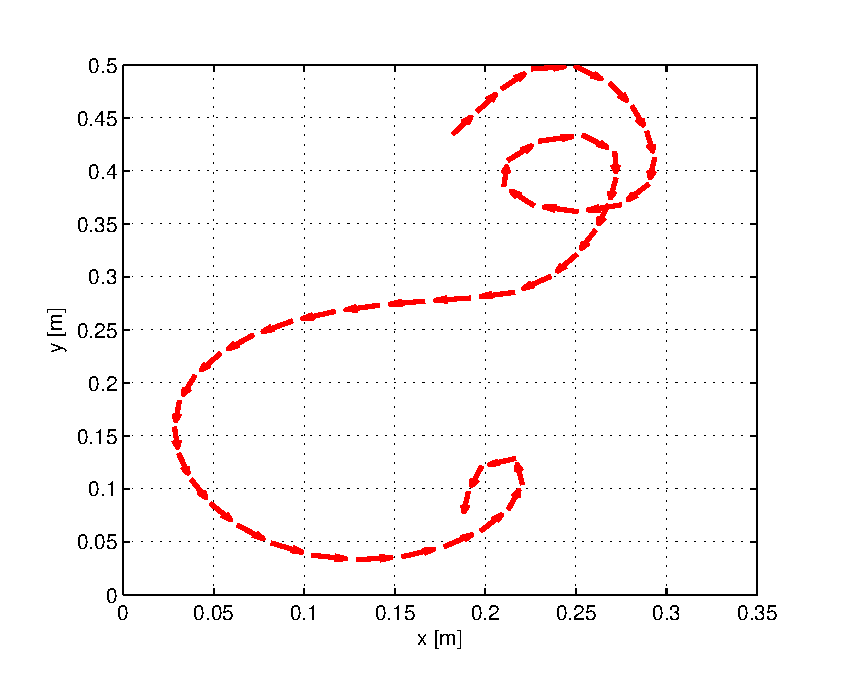
\includegraphics[width=0.5\textwidth]{Figures/Lagrangian_trajectory}
\caption{Trajectory of an independent particle in turbulence.}
\label{fig:lag_traj}
\end{figure}

An example of the connected particle system is the spring mass model \cite{blickhan1989spring}, which can effectively simulate the behavior of elastic material, such as cloth\cite{Baraff1998Large}, muscle \cite{NedelReal1998} and skin\cite{GelderApproximate1998} etc. A simulation of parachute in turbulent flow using spring-mass model is displayed in \Fig{fig:spring_mesh}. 
\begin{figure}
\centering
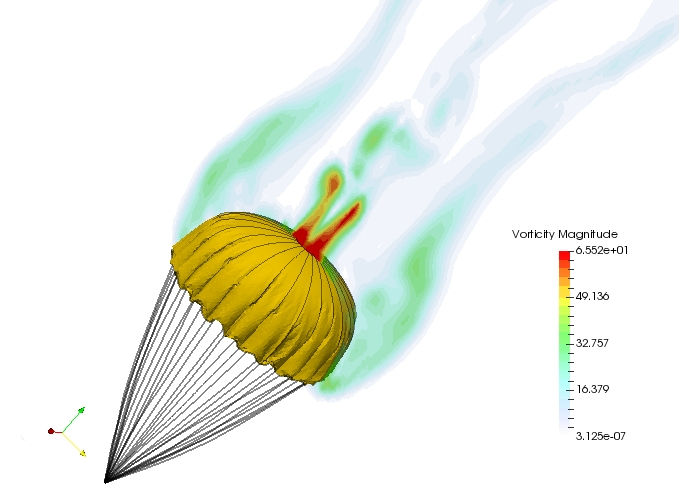
\includegraphics[width=0.5\textwidth]{Figures/parachute_turb.jpg} 
\caption{Simulation of parachute in turbulent flow using spring-mass system.} 
\label{fig:spring_mesh}
\end{figure}
In mathematics, the velocity $\vect{v}$ and position $\vect{x}$ of $n$ particles are determined by:
\begin{equation}
\dot{\vect{x}} = \vect{v}
\label{spring_x_eqn}
\end{equation}
\begin{equation}
\dot{\vect{v}} = \vect{M}^{-1}(\vect{f}_i
				+ \vect{f}_d + \vect{f}_e \label{spring_v_eqn})
\end{equation}
where $\vect{f}_i = -\frac{\partial W}{\partial \vect{x}_i}$ is the internal force restoring the surface deformation and $W$ is a scalar function of $\vect{x}$ describing the cloth internal energy; diagonal matrix $\vect{M} \in \mathbb{R}^{3n\times 3n}$ represents the mass distribution of the cloth; $\vect{f}_d$ is the damping function that will be discussed later; $\vect{f}_e$ is the external force (such as air-drag, gravity, contact constrains, etc.) acting on the cloth. This model is well defined if the energy function $W$ for each mass point is specified. In fact, the elastic membrane can be discretized into triangles and then the potential energy in a deformed triangle consists of two parts: the energy of three tensile springs that prevent edges from stretching; the energy of three angular springs that prevent any change of vertex angles. Intuitively, the formula of $W$ for the $i$-th particle should include all the particles connecting to it. The specific form of $W$ will be introduced in later chapter.

In the next chapter, the numerical methods for solving Navier-Stokes equation, convection-diffusion-reaction equation and particle system are introduced. In fact, these equations can be solved using various numerical methods, which have their own advantages and disadvantages comparing with each other. These will be discussed in details in the next chapter.
